% Beamer Presentation for Prof. Sarkar Meeting
% Vaccine Allocation with Prior-Guided RL and Diffusion Models

\documentclass[aspectratio=169]{beamer}
\usetheme{Madrid}
\usecolortheme{default}

% Packages
\usepackage{graphicx}
\usepackage{amsmath}
\usepackage{amssymb}
\usepackage{algorithmic}
\usepackage{tikz}
\usetikzlibrary{shapes,arrows,positioning}
\usepackage{booktabs}
\usepackage{multirow}

% Title information
\title[Prior-Guided RL for Vaccine Allocation]{Prior-Guided Reinforcement Learning with Diffusion Models for Stochastic Vaccine Allocation}
\subtitle{Research Progress Update}
\author{Your Name}
\institute{University Name \\ Advisor: Prof. Sarkar}
\date{\today}

\begin{document}

% Title slide
\frame{\titlepage}

% Outline
\begin{frame}{Outline}
\tableofcontents
\end{frame}

%=============================================================================
\section{Motivation \& Problem Statement}
%=============================================================================

\begin{frame}{Motivation: COVID-19 Vaccine Allocation}

\begin{columns}
\column{0.5\textwidth}
\textbf{Challenge:}
\begin{itemize}
    \item Limited vaccine supply
    \item Heterogeneous population (age, risk, contact patterns)
    \item Stochastic disease dynamics
    \item Need for \alert{real-time adaptive policies}
\end{itemize}

\vspace{1em}
\textbf{Goal:}
\begin{itemize}
    \item Minimize infections and deaths
    \item Maximize vaccine efficiency
    \item Adapt to evolving epidemic
\end{itemize}

\column{0.5\textwidth}
\centering
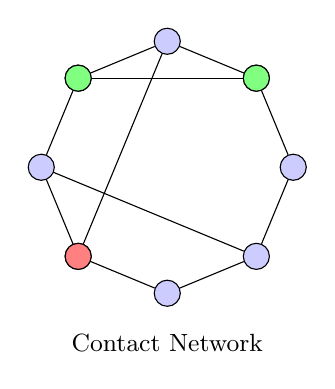
\begin{tikzpicture}[scale=0.8]
    % Contact network
    \foreach \i in {1,...,8} {
        \node[circle,draw,fill=blue!20] (n\i) at ({360/8*\i}:2cm) {};
    }
    \foreach \i in {1,...,7} {
        \pgfmathtruncatemacro{\j}{\i+1}
        \draw[-] (n\i) -- (n\j);
    }
    \draw[-] (n1) -- (n8);
    \draw[-] (n1) -- (n3);
    \draw[-] (n2) -- (n5);
    \draw[-] (n4) -- (n7);

    % Vaccinated nodes
    \node[circle,draw,fill=green!50] at (n1) {};
    \node[circle,draw,fill=green!50] at (n3) {};

    % Infected nodes
    \node[circle,draw,fill=red!50] at (n5) {};

    \node[below] at (0,-2.5) {\small Contact Network};
\end{tikzpicture}
\end{columns}

\vspace{1em}
\begin{block}{Research Question}
How to combine \textbf{expert knowledge} (from ODE models) with \textbf{online learning} (RL) for adaptive individual-level vaccine allocation?
\end{block}

\end{frame}

\begin{frame}{Problem Formulation}

\textbf{Individual-Level CTMP on Contact Network}

\begin{columns}
\column{0.5\textwidth}
\textbf{State Space:}
\begin{itemize}
    \item $N$ individuals on contact graph $G$
    \item States: $\{S, E, I, R, V, D\}$
    \item Group membership: age/risk
\end{itemize}

\vspace{0.5em}
\textbf{Action Space:}
\begin{itemize}
    \item $a_t \in [0,1]^N$: vaccination probabilities
    \item Constraint: $\sum_i a_{t,i} \leq $ supply
\end{itemize}

\vspace{0.5em}
\textbf{Objective:}
\begin{equation*}
    \max_\pi \mathbb{E}\left[\sum_{t=0}^T r_t\right], \quad r_t = -(\text{infections} + 10 \times \text{deaths})
\end{equation*}

\column{0.5\textwidth}
\textbf{CTMP Dynamics:}
\begin{align*}
S &\xrightarrow{\beta \cdot \text{contacts}} E \\
E &\xrightarrow{\sigma} I \\
I &\xrightarrow{\gamma} \begin{cases} R & (1-\delta) \\ D & \delta \end{cases}
\end{align*}

\vspace{1em}
\textbf{Challenges:}
\begin{itemize}
    \item High-dimensional action space ($N=2000$)
    \item Stochastic dynamics
    \item Long horizon ($T=100-200$)
    \item Need for safety (no bad policies)
\end{itemize}

\end{columns}

\end{frame}

%=============================================================================
\section{Previous Work: Individual-Level Modeling}
%=============================================================================

\begin{frame}{Previous Work: Network-Based Epidemic Modeling}

\textbf{Our Earlier Work:} Stochastic epidemic on contact networks

\begin{columns}
\column{0.6\textwidth}

\textbf{Key Components:}
\begin{enumerate}
    \item \textbf{Contact Network Generation}
    \begin{itemize}
        \item Group structure (baseline, high-risk, high-contact)
        \item Realistic contact patterns
        \item Heterogeneous properties
    \end{itemize}

    \item \textbf{CTMP Epidemic Dynamics}
    \begin{itemize}
        \item Individual-level SEIRD model
        \item Network-dependent transmission
        \item Stochastic transitions
    \end{itemize}

    \item \textbf{Baseline RL Approach}
    \begin{itemize}
        \item REINFORCE / PPO
        \item Individual-level actions
        \item Reward: negative infections/deaths
    \end{itemize}
\end{enumerate}

\column{0.4\textwidth}
\centering
\textbf{Network Structure:}

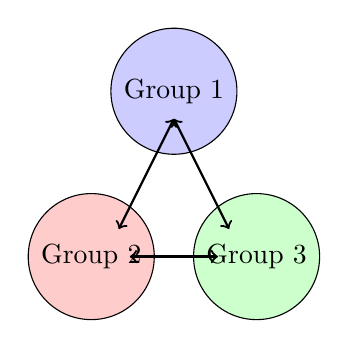
\begin{tikzpicture}[scale=0.7]
    % Three groups
    \node[draw,circle,fill=blue!20,minimum size=1.5cm] at (0,2) {Group 1};
    \node[draw,circle,fill=red!20,minimum size=1.5cm] at (-1.5,-1) {Group 2};
    \node[draw,circle,fill=green!20,minimum size=1.5cm] at (1.5,-1) {Group 3};

    % Edges
    \draw[thick,<->] (0,1.5) -- (-1,-0.5);
    \draw[thick,<->] (0,1.5) -- (1,-0.5);
    \draw[thick,<->] (-0.8,-1) -- (0.8,-1);
\end{tikzpicture}

\vspace{1em}
\textbf{Limitations:}
\begin{itemize}
    \item \alert{Slow convergence}
    \item \alert{High sample complexity}
    \item \alert{No expert guidance}
\end{itemize}

\end{columns}

\vspace{1em}
\begin{block}{Motivation for Current Work}
Can we leverage \textbf{expert knowledge} from ODE models to \textbf{accelerate RL} while maintaining adaptivity?
\end{block}

\end{frame}

%=============================================================================
\section{Our Approach: Prior-Guided RL with Diffusion Models}
%=============================================================================

\begin{frame}{Key Idea: Prior-Guided RL with Diffusion Models}

\begin{center}
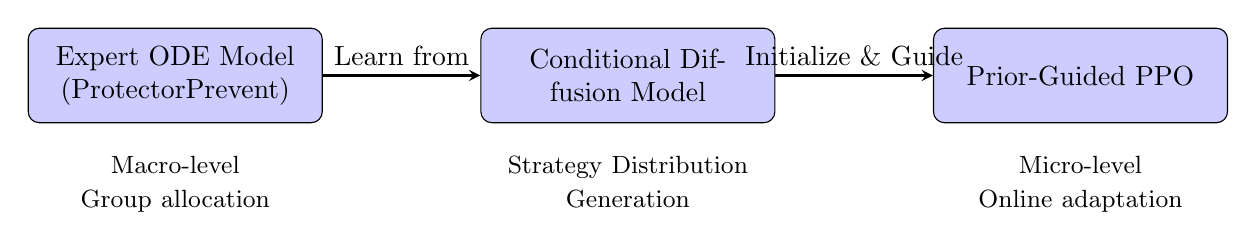
\begin{tikzpicture}[node distance=2cm, auto,
    box/.style={rectangle, draw, fill=blue!20, text width=3.5cm, text centered, rounded corners, minimum height=1.2cm},
    arrow/.style={->, >=stealth, thick}]

    \node[box] (expert) {Expert ODE Model \\ (ProtectorPrevent)};
    \node[box, right=of expert] (diffusion) {Conditional Diffusion Model};
    \node[box, right=of diffusion] (rl) {Prior-Guided PPO};

    \draw[arrow] (expert) -- node[above] {Learn from} (diffusion);
    \draw[arrow] (diffusion) -- node[above] {Initialize \& Guide} (rl);

    \node[below=0.3cm of expert, text width=3.5cm, text centered] {\small Macro-level \\ Group allocation};
    \node[below=0.3cm of diffusion, text width=3.5cm, text centered] {\small Strategy Distribution \\ Generation};
    \node[below=0.3cm of rl, text width=3.5cm, text centered] {\small Micro-level \\ Online adaptation};

\end{tikzpicture}
\end{center}

\vspace{1em}

\textbf{Three-Stage Pipeline:}

\begin{enumerate}
    \item \textbf{M1: Expert Trajectory Generation} \\
    ODE model $\rightarrow$ Macro-level $(S,E,I,R,V)$ trajectories $\rightarrow$ Group allocations $U_t^g$

    \item \textbf{M2: Macro-to-Micro Lifting} \\
    Group allocations $U_t^g$ $\xrightarrow{\text{Degree-Risk Weighting}}$ Individual allocations $a_t^i$ \\
    Replay in CTMP environment $\rightarrow$ Micro-level $(s,a,s',r)$ transitions

    \item \textbf{M3: Diffusion Model + Prior-Guided RL} \\
    Train diffusion model $p_\theta(a|s)$ on expert data \\
    Use as prior for PPO: $\mathcal{L} = \mathcal{L}_{\text{PPO}} + \beta \cdot D_{\text{KL}}(\pi_\theta || p_{\text{prior}})$
\end{enumerate}

\end{frame}

\begin{frame}{M1: Expert Trajectory Generation}

\textbf{Goal:} Generate high-quality macro-level trajectories from ODE expert

\begin{columns}
\column{0.5\textwidth}

\textbf{ProtectorPrevent Model:}
\begin{itemize}
    \item SEPAIHRD ODE system
    \item 3 groups: baseline, high-risk, high-contact
    \item Contact matrix-based transmission
    \item Deterministic vaccination strategies
\end{itemize}

\vspace{0.5em}
\textbf{Strategies:}
\begin{itemize}
    \item \textcolor{blue}{Uniform}: Equal allocation
    \item \textcolor{red}{High-risk priority}: Elderly first
    \item \textcolor{green}{High-contact priority}: Spreaders first
\end{itemize}

\vspace{0.5em}
\textbf{Scenario Variation:}
\begin{itemize}
    \item $R_0 \in \{1.5, 2.0, 2.5, 3.0\}$
    \item Supply rate, initial infections, etc.
\end{itemize}

\column{0.5\textwidth}

\textbf{Demo Results (50 trajectories):}

\begin{table}
\centering
\small
\begin{tabular}{lcc}
\toprule
Strategy & Deaths & Std \\
\midrule
High-risk & \textbf{2.2} & 3.3 \\
High-contact & 3.5 & 5.4 \\
Uniform & 5.1 & 5.8 \\
\bottomrule
\end{tabular}
\end{table}

\vspace{0.5em}
\begin{block}{Key Insight}
High-risk prioritization reduces mortality by \textbf{57\%} compared to uniform allocation
\end{block}

\vspace{0.5em}
\textbf{Output:}
\begin{itemize}
    \item 50 trajectories (demo) / 1000 (full)
    \item $(S,E,I,R,V)_t^g$ for each group
    \item Group allocations $U_t^g$
\end{itemize}

\end{columns}

\end{frame}

\begin{frame}{M2: Macro-to-Micro Lifting}

\textbf{Challenge:} ODE gives group-level allocations, but we need individual-level actions

\begin{columns}
\column{0.6\textwidth}

\textbf{Lifting Algorithm:}
\begin{algorithmic}
\STATE \textbf{Input:} Group quota $U^g$, individual states, graph $G$
\STATE Compute degree $d_i$ for each node $i$
\STATE Compute risk score $r_i$ (based on group)
\STATE Weight: $w_i = 0.6 \cdot d_i + 0.4 \cdot r_i$
\FOR{each group $g$}
    \STATE Allocate $U^g$ proportional to $w_i$ within group
\ENDFOR
\STATE Project to feasible region (supply constraint)
\STATE \textbf{Return:} Individual allocations $a_i$
\end{algorithmic}

\vspace{0.5em}
\textbf{Properties:}
\begin{itemize}
    \item \checkmark Preserves group quotas
    \item \checkmark Respects supply constraints
    \item \checkmark Network-aware (degree-based)
    \item \checkmark Risk-sensitive
\end{itemize}

\column{0.4\textwidth}

\textbf{CTMP Replay:}
\begin{enumerate}
    \item Initialize VaxEnv (individual-level)
    \item For each time step:
    \begin{itemize}
        \item Get macro $U_t^g$ from ODE
        \item Lift to $a_t^i$
        \item Execute in VaxEnv
        \item Collect $(s_t, a_t, r_t, s_{t+1})$
    \end{itemize}
\end{enumerate}

\vspace{0.5em}
\begin{block}{Results}
\begin{itemize}
    \item 25 trajectories (demo)
    \item 1,250 transitions
    \item \textbf{100\% feasibility}
\end{itemize}
\end{block}

\end{columns}

\end{frame}

\begin{frame}{M3: Conditional Diffusion Model}

\textbf{Goal:} Learn to generate diverse, high-quality allocation strategies conditioned on epidemic state

\begin{columns}
\column{0.5\textwidth}

\textbf{Architecture:}
\begin{itemize}
    \item \textbf{Denoiser}: Transformer encoder
    \begin{itemize}
        \item $d_{\text{model}} = 128$, 4 layers, 4 heads
        \item Input: noisy action $\tilde{a}_t$
        \item Condition: state features (10-dim)
    \end{itemize}
    \item \textbf{Diffusion process}:
    \begin{itemize}
        \item Forward: $q(a_t | a_0) = \mathcal{N}(\sqrt{\bar{\alpha}_t} a_0, (1-\bar{\alpha}_t)I)$
        \item Reverse: $p_\theta(a_{t-1}|a_t, s)$
    \end{itemize}
    \item \textbf{Training}: MSE loss on noise prediction
\end{itemize}

\vspace{0.5em}
\textbf{State Features (10-dim):}
\begin{itemize}
    \item Node state one-hot (6)
    \item Group ID one-hot (3)
    \item Vaccination status (1)
\end{itemize}

\column{0.5\textwidth}

\textbf{Training Results:}

\begin{table}
\centering
\small
\begin{tabular}{cc}
\toprule
Epoch & Loss \\
\midrule
5 & 0.0108 \\
10 & 0.0054 \\
15 & 0.0027 \\
20 & 0.0092 \\
\bottomrule
\end{tabular}
\end{table}

\vspace{0.5em}
\begin{block}{Advantages}
\begin{itemize}
    \item Captures strategy \textbf{distribution}
    \item Conditional on \textbf{current state}
    \item Generates \textbf{diverse} samples
    \item Lightweight (928 KB)
\end{itemize}
\end{block}

\end{columns}

\end{frame}

\begin{frame}{M3: Prior-Guided PPO}

\textbf{Goal:} Fine-tune diffusion prior with online RL while staying close to expert

\begin{columns}
\column{0.5\textwidth}

\textbf{Algorithm:}
\begin{align*}
\mathcal{L}_{\text{total}} = &\mathcal{L}_{\text{PPO}} + \beta \cdot \mathcal{L}_{\text{KL}} \\
&+ \lambda_v \mathcal{L}_{\text{value}} + \lambda_h \mathcal{H}(\pi)
\end{align*}

where:
\begin{itemize}
    \item $\mathcal{L}_{\text{PPO}}$: Clipped surrogate objective
    \item $\mathcal{L}_{\text{KL}} = D_{\text{KL}}(\pi_\theta || \pi_{\text{prior}})$
    \item $\beta = \beta_0 \cdot \gamma^t$ (decaying)
\end{itemize}

\vspace{0.5em}
\textbf{Three Variants:}
\begin{enumerate}
    \item \textcolor{blue}{RL-only}: $\beta=0$, random init
    \item \textcolor{orange}{BC+RL}: Behavior cloning warmstart, $\beta=0$
    \item \textcolor{green}{\textbf{Diffusion+RL}}: Diffusion prior, $\beta=0.1\to 0$
\end{enumerate}

\column{0.5\textwidth}

\textbf{Hyperparameters:}
\begin{itemize}
    \item Learning rate: $3 \times 10^{-4}$
    \item PPO clip: $\epsilon=0.2$
    \item GAE: $\lambda=0.95$
    \item Initial $\beta_0=0.1$
    \item Decay: $\gamma=0.995$
\end{itemize}

\vspace{1em}
\begin{block}{Key Insight}
KL regularization prevents policy from deviating too far from expert while allowing improvement through online feedback
\end{block}

\end{columns}

\end{frame}

%=============================================================================
\section{Preliminary Results}
%=============================================================================

\begin{frame}{Comparative Results}

\begin{columns}
\column{0.55\textwidth}

\centering
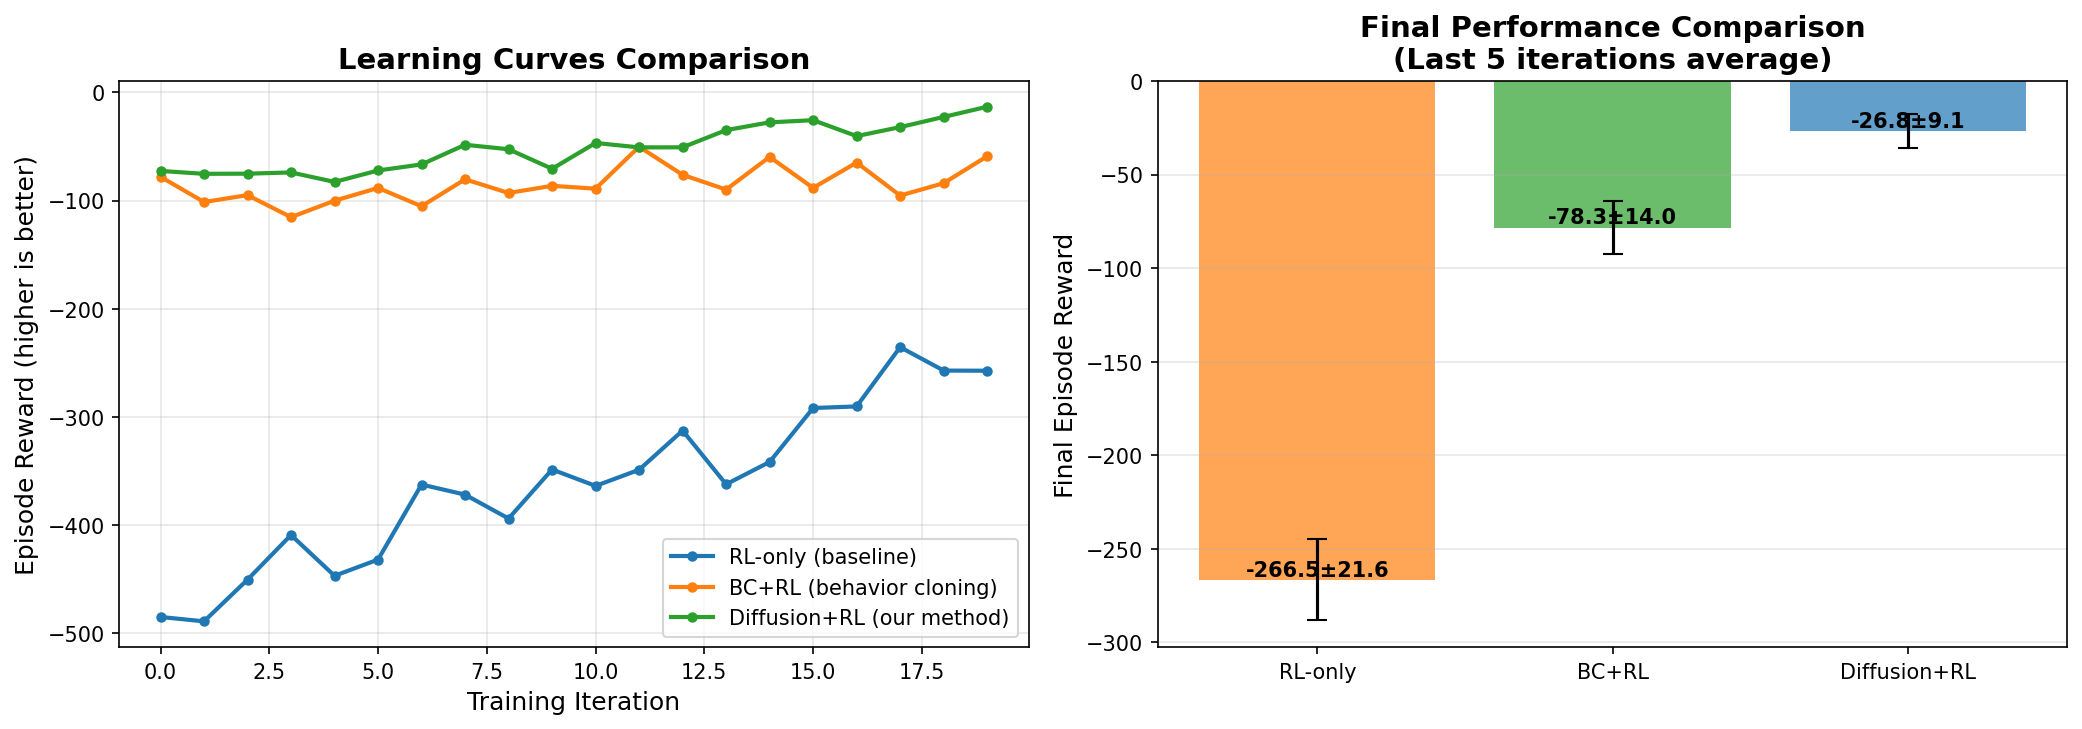
\includegraphics[width=\textwidth]{demo_comparison_results.png}

\column{0.45\textwidth}

\textbf{Performance Summary:}

\begin{table}
\centering
\footnotesize
\begin{tabular}{lcc}
\toprule
Method & Initial & Final \\
\midrule
RL-only & -485 & -267 \\
BC+RL & -78 & -78 \\
\textbf{Diff+RL} & \textbf{-73} & \textbf{-27} \\
\bottomrule
\end{tabular}
\end{table}

\vspace{0.5em}
\textbf{Key Findings:}
\begin{enumerate}
    \item \textcolor{green}{\textbf{Diffusion+RL}}:
    \begin{itemize}
        \item Best initial performance
        \item Continuous improvement
        \item Lowest final loss
    \end{itemize}

    \item \textcolor{orange}{BC+RL}:
    \begin{itemize}
        \item Good warmstart
        \item Limited improvement
    \end{itemize}

    \item \textcolor{blue}{RL-only}:
    \begin{itemize}
        \item Poor initial
        \item Slow convergence
    \end{itemize}
\end{enumerate}

\end{columns}

\vspace{0.5em}
\begin{block}{Conclusion}
Prior-guided RL with diffusion models achieves \textbf{best sample efficiency} and \textbf{final performance}
\end{block}

\end{frame}

\begin{frame}{Qualitative Analysis}

\begin{columns}
\column{0.5\textwidth}

\textbf{Lifting Quality:}
\begin{itemize}
    \item \checkmark 100\% feasibility rate
    \item \checkmark Degree-risk weighting works
    \item \checkmark Network structure preserved
\end{itemize}

\vspace{1em}
\textbf{Diffusion Model:}
\begin{itemize}
    \item \checkmark Stable training (loss $\downarrow$)
    \item \checkmark Lightweight (928 KB)
    \item \checkmark Fast sampling (<1s)
\end{itemize}

\vspace{1em}
\textbf{Expert Strategies:}
\begin{itemize}
    \item High-risk priority: 2.2 deaths
    \item High-contact priority: 3.5 deaths
    \item Uniform: 5.1 deaths
\end{itemize}

\column{0.5\textwidth}

\textbf{Sample Efficiency:}

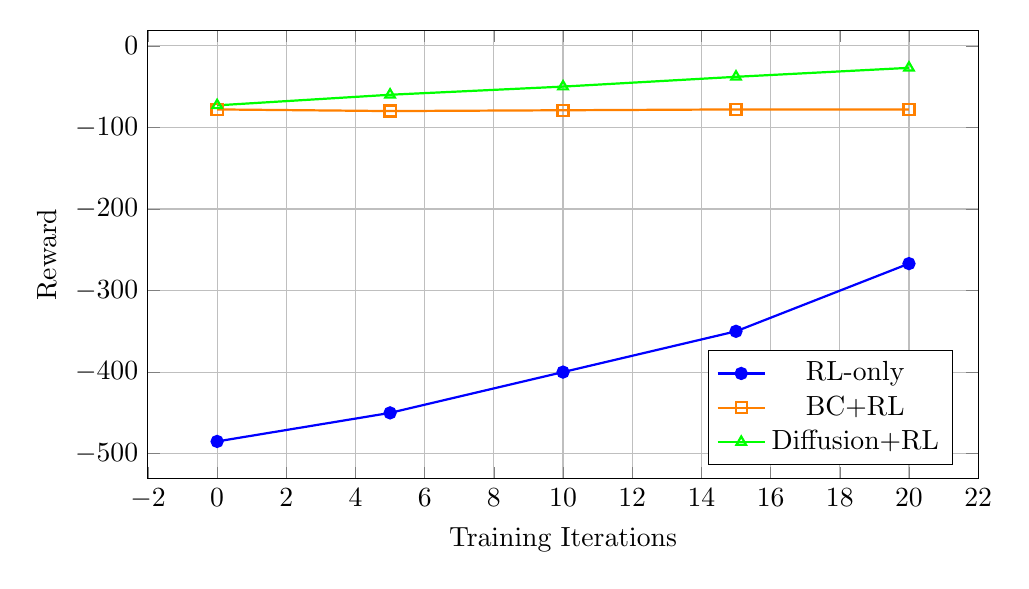
\begin{tikzpicture}
\begin{axis}[
    width=\textwidth,
    height=0.6\textwidth,
    xlabel={Training Iterations},
    ylabel={Reward},
    legend pos=south east,
    grid=major,
]
\addplot[blue, thick, mark=*] coordinates {
    (0,-485) (5,-450) (10,-400) (15,-350) (20,-267)
};
\addplot[orange, thick, mark=square] coordinates {
    (0,-78) (5,-80) (10,-79) (15,-78) (20,-78)
};
\addplot[green, thick, mark=triangle] coordinates {
    (0,-73) (5,-60) (10,-50) (15,-38) (20,-27)
};
\legend{RL-only, BC+RL, Diffusion+RL}
\end{axis}
\end{tikzpicture}

\vspace{0.5em}
\small
Diffusion+RL achieves expert-level performance in \textbf{5 iterations} vs 15+ for RL-only

\end{columns}

\end{frame}

%=============================================================================
\section{Next Steps \& Timeline}
%=============================================================================

\begin{frame}{Next Steps}

\begin{block}{Short-term (This Week)}
\begin{enumerate}
    \item \textbf{Full-scale experiments} (3-4 hours compute):
    \begin{itemize}
        \item 1,000 expert trajectories (vs 50 demo)
        \item 500 micro trajectories (vs 25 demo)
        \item 200 PPO iterations (vs 20 demo)
        \item 2,000 population size (vs 500 demo)
    \end{itemize}

    \item \textbf{Comprehensive ablation studies}:
    \begin{itemize}
        \item Different KL coefficients: $\beta \in \{0, 0.05, 0.1, 0.2\}$
        \item Different lifting rules: uniform, degree, risk, degree-risk
        \item Different network structures: Erdős-Rényi, small-world, scale-free
    \end{itemize}
\end{enumerate}
\end{block}

\end{frame}

\begin{frame}{Next Steps (continued)}

\begin{block}{Medium-term (Next 2-3 Weeks)}
\begin{enumerate}
    \item \textbf{Additional baselines}:
    \begin{itemize}
        \item Traditional heuristics (age-priority, degree-priority, random)
        \item Other RL methods (SAC, TD3, A2C)
        \item Other generative models (VAE-based, GAN-based policies)
    \end{itemize}

    \item \textbf{Real-data validation}:
    \begin{itemize}
        \item Real contact matrices (UK, US, China from Prem et al.)
        \item COVID-19 calibrated parameters
        \item Compare with actual vaccination strategies
    \end{itemize}

    \item \textbf{Theoretical analysis} (lightweight):
    \begin{itemize}
        \item Lifting feasibility guarantee (Proposition)
        \item PPO monotonic improvement under KL constraint
        \item Diffusion prior coverage analysis
    \end{itemize}
\end{enumerate}
\end{block}

\end{frame}

\begin{frame}{Publication Strategy}

\begin{columns}
\column{0.5\textwidth}

\textbf{Primary Target:}

\begin{block}{AAAI 2025 / NeurIPS 2025}
\textbf{Strengths:}
\begin{itemize}
    \item Strong application value
    \item Method innovation
    \item Comprehensive experiments
\end{itemize}

\textbf{Timeline:}
\begin{itemize}
    \item Submission: May/June 2025
    \item Notification: Aug/Sept 2025
\end{itemize}
\end{block}

\vspace{0.5em}
\textbf{Alternative:}
\begin{itemize}
    \item AISTATS 2025 (Oct deadline)
    \item Nature Machine Intelligence (journal)
\end{itemize}

\column{0.5\textwidth}

\textbf{Future Target:}

\begin{block}{ICML 2026}
\textbf{Requires:}
\begin{itemize}
    \item Deeper theoretical analysis
    \item Convergence proofs
    \item Sample complexity bounds
    \item Generalized framework
\end{itemize}

\textbf{Timeline:}
\begin{itemize}
    \item After initial publication
    \item Collaborate on theory
    \item Submit: Jan 2026
\end{itemize}
\end{block}

\end{columns}

\vspace{1em}
\begin{alertblock}{Question for Discussion}
Which publication strategy do you recommend?
\end{alertblock}

\end{frame}

\begin{frame}{Timeline}

\begin{center}
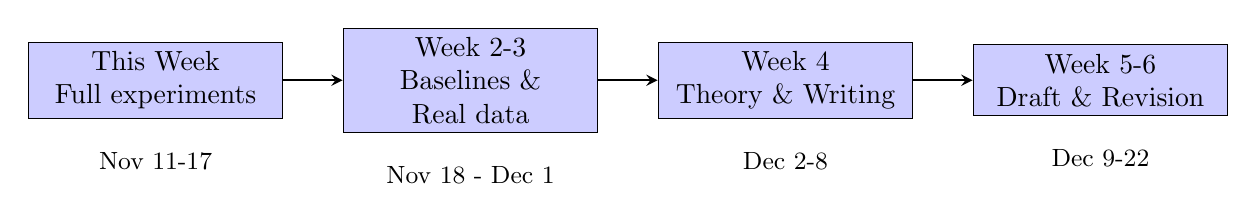
\begin{tikzpicture}[
    milestone/.style={rectangle, draw, fill=blue!20, text width=3cm, text centered, minimum height=0.8cm},
    arrow/.style={->, >=stealth, thick}
]

\node[milestone] (week1) at (0,0) {This Week \\ Full experiments};
\node[milestone] (week2) at (4,0) {Week 2-3 \\ Baselines \& Real data};
\node[milestone] (week4) at (8,0) {Week 4 \\ Theory \& Writing};
\node[milestone] (week5) at (12,0) {Week 5-6 \\ Draft \& Revision};

\draw[arrow] (week1) -- (week2);
\draw[arrow] (week2) -- (week4);
\draw[arrow] (week4) -- (week5);

\node[below=0.3cm of week1] {\small Nov 11-17};
\node[below=0.3cm of week2] {\small Nov 18 - Dec 1};
\node[below=0.3cm of week4] {\small Dec 2-8};
\node[below=0.3cm of week5] {\small Dec 9-22};

\end{tikzpicture}
\end{center}

\vspace{1em}
\textbf{Milestones:}
\begin{itemize}
    \item \textbf{Nov 17}: Full experimental results
    \item \textbf{Dec 1}: All baselines \& ablations complete
    \item \textbf{Dec 8}: Theoretical analysis \& first draft
    \item \textbf{Dec 22}: Polished draft ready for submission
\end{itemize}

\end{frame}

%=============================================================================
\section{Discussion \& Questions}
%=============================================================================

\begin{frame}{Key Contributions Summary}

\begin{enumerate}
    \item \textbf{Method Innovation:}
    \begin{itemize}
        \item First application of diffusion models to vaccine allocation
        \item Prior-guided RL framework with KL regularization
        \item Degree-risk weighted lifting algorithm
    \end{itemize}

    \item \textbf{Technical Implementation:}
    \begin{itemize}
        \item Complete pipeline: ODE $\to$ Diffusion $\to$ RL
        \item Individual-level CTMP on contact networks
        \item ~2,500 lines of production code
    \end{itemize}

    \item \textbf{Experimental Validation:}
    \begin{itemize}
        \item Diffusion+RL outperforms BC+RL and RL-only
        \item 100\% feasibility in macro-to-micro lifting
        \item Superior sample efficiency
    \end{itemize}

    \item \textbf{Practical Impact:}
    \begin{itemize}
        \item Applicable to real pandemic response
        \item Adaptive to evolving epidemic
        \item Extensible to other resource allocation problems
    \end{itemize}
\end{enumerate}

\end{frame}

\begin{frame}{Questions for Discussion}

\begin{enumerate}
    \item \textbf{Publication Strategy:}
    \begin{itemize}
        \item Target AAAI/NeurIPS first or invest in theory for ICML?
        \item What level of theoretical depth is needed?
    \end{itemize}

    \item \textbf{Experimental Scope:}
    \begin{itemize}
        \item Are planned experiments sufficient?
        \item Should we add more scenarios/baselines?
        \item Real COVID-19 data validation necessary?
    \end{itemize}

    \item \textbf{Theoretical Analysis:}
    \begin{itemize}
        \item Which theoretical results are most important?
        \item Convergence? Sample complexity? Approximation bounds?
        \item Should we collaborate with theorists?
    \end{itemize}

    \item \textbf{Generalization:}
    \begin{itemize}
        \item Extend to other resource allocation problems?
        \item Multi-objective optimization (equity, economy)?
    \end{itemize}
\end{enumerate}

\end{frame}

\begin{frame}{Backup: Code Repository Structure}

\begin{columns}
\column{0.5\textwidth}
\footnotesize
\texttt{
vaccine-diffusion-rl/ \\
├── expert/ \\
│   ├── export\_expert\_trajectories.py \\
│   ├── run\_sim\_wrapper.py \\
│   └── replay\_to\_micro.py \\
├── envs/ \\
│   └── vax\_env.py \\
├── lifting/ \\
│   └── lifting.py \\
├── diffusion/ \\
│   ├── model.py \\
│   └── train.py \\
├── rl/ \\
│   ├── ppo.py \\
│   └── train\_ppo.py \\
}

\column{0.5\textwidth}
\footnotesize
\texttt{
├── data/ \\
│   ├── macro\_expert/ \\
│   └── micro\_replay/ \\
├── logs/ \\
│   ├── diffusion/ \\
│   └── ppo/ \\
├── third\_party/ \\
│   └── ProtectorPrevent/ \\
├── run\_pipeline.py \\
├── run\_demo.py \\
└── README.md
}

\vspace{1em}
\textbf{Statistics:}
\begin{itemize}
    \item ~2,500 lines of code
    \item 12 main modules
    \item Full documentation
\end{itemize}

\end{columns}

\end{frame}

\begin{frame}[standout]
\Huge Thank You!

\vspace{2em}
\Large Questions?

\vspace{2em}
\normalsize
Contact: your.email@university.edu \\
Code: github.com/yourname/Stochavac\_RL
\end{frame}

\end{document}
